%% Lee
%% In dissertation, change section* to chapter and subsection* to section


\chapter{Three-Dimensional Integrated Circuits (3DIC)}
\label{chap-three}

Over the last couple of decades, the ever shrinking world of \acp{ic} has enabled the introduction of devices society takes for granted such as personal computing and cell phones.

As \ac{ic} technology has shrunk, design complexity has grown to take advantage where hundreds of millions of transistors are placed on a typical \ac{ic}.
These \acp{ic} have evolved from performing small functions to becoming systems on a chip.

However, at some point, an \ac{ic} has to interface with another function and often that communication involves the moving of data to and from memory and the increase in complexity often drives a need for higher memory data bandwidth. 

The \ac{ic} complexity has been doubling approximately every two years but the external interfaces are restricted by physical limitations.
Within the \ac{soc}, the designer can take advantage of very wide interfaces, often thousands of bits wide to increase bandwidth, but when data is moved to off-chip memory, the widest buses are usually hundreds of bits wide.

One way to avoid this limitation is to employ \ac{3dic} (see figure \ref{fig:3DIC Die}). The advantages of \ac{3dic} are well understood. reducing the amount of off-chip communication increases bandwidth and reduces power. The power reduction comes from not having to drive the relatively
high capacitance inputs and outputs.

\begin{figure}
\centering
\begin{subfigure}{.8\textwidth}
  \centering
  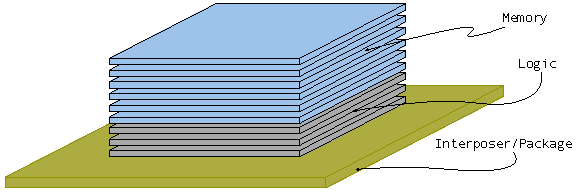
\includegraphics[width=1\textwidth]{DieStack}
  \captionsetup{justification=centering, skip=5pt}
  \caption{Different Die types stacked mounted on an interposer/package substrate}
  \label{fig:Die Stack}
\end{subfigure}%

\bigskip

\begin{subfigure}{.8\textwidth}
  \centering
  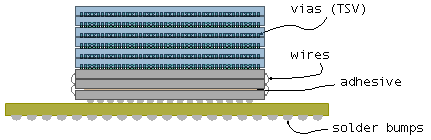
\includegraphics[width=1\textwidth]{DieStackConnections}
  \captionsetup{justification=centering, skip=5pt}
  \caption{Connection Types}
  \label{fig:Die Stack Connection Types}
\end{subfigure}
\captionsetup{justification=centering, skip=12pt}
\caption[3DIC Stack of Die]{3DIC Stack of Die}
\label{fig:3DIC Die}
\end{figure}

Taking advantage of \ac{3dic} means stacking die on top of one another and making connections directly between the die. These connections can be in the form of wire made at the edges of the die or using vias buried in the die itself.


Below is a summary the benefits of \ac{3dic} :
\begin{outline}
  \1 Reduced Power
    \2 mainly from not having to drive external outputs and receiving external inputs
  \1 Increased Connectivity
    \2 maintaining very wides buses through the \ac{soc} increases bandwidth
  \1 Ability to mix heterogeneous technology
    \2 Mixed Analog/Digital
    \2 Mixing memory technology and logic technology
  \1 Increase density and mitigation against the slowing of Moores Law
    \2 using the vertical domain to increase perceived transistor per $mm^2$
  \1 Potentially lower costs by combining simpler die rather than build a large die
    \2 yield benefits from combining higher yield die
  \1 Possibility of novel architectures \cite{Kim2016}
\end{outline}

Some disadvantages of \ac{3dic} are:
\begin{outline}
  \1 Reliability
  \1 Cost
    \2 being a relatively new technology it is still expensive 
    \2 \ac{tsv} technology is still unreliable
\end{outline}

There is still some reluctance to fully embrace \ac{3dic} but undoubtly the various barriers will be broken down.

The ability to mix heterogenous technology is of particular interest to this works target application because mixing technology targeted toward \ac{dram} with cmos logic technology is a heterogenous mix of which this work takes advantage.

In \cite{itrs2015_interconn} there are four definitions of \ac{3dic} interconnects:

\begin{outline}
%\section{3D-Wafer level package \cite{itrs2015_interconn}}
%\label{sec:3D-Wafer level package}

  \1 3D-Wafer level package \cite{itrs2015_interconn}
    \2 In this case, different die are stacked and then connected using traditional bond bumps and/or bond wires at the periphery of the chip.
    \2 This technique provides better transistor density compared to traditional 2D-IC with improvements in interconnect density.

%\section{3D-Stacked SoC\ac{soc} \cite{itrs2015_interconn}}
%\label{sec:3D-Stacked \ac{soc}}
  \1 3D-Stacked \ac{soc} \cite{itrs2015_interconn}
    \2 In this case, different die are stacked and then connected using \acp{tsv}. The \acp{tsv} connect the dies to intermediate metal layers known as global metal layers. This allows the indivial die to maintain a high level of functionality and thus is similar to connecting functional building blocks meaning the individual die are likely to be significant functional pieces of \ac{ip}.
    \2 using \acp{tsv} provides a medium level of interconnect

%\section{3D-Stack \ac{ic} \cite{itrs2015_interconn}}
%\label{sec:3D-Stack \ac{ic}}
  \1 3D-Stack \ac{ic} \cite{itrs2015_interconn}
    \2 In this case, different die are stacked and then connected using \acp{tsv}. The \acp{tsv} connect the dies to intermediate higher metal layers known as global metal layers. This infers the individual die are not large functioning pieces of \ac{ip}.
    \2 using \acp{tsv} provides a high level of interconnect

%\section{3D-Integrated Circuit \cite{itrs2015_interconn}}
%\label{sec:3D-Integrated Circuit}
  \1 3D-Integrated Circuit \cite{itrs2015_interconn}
    \2 In this case there are not multiple dies. Instead the additional silicon layers are deposited on top of each other with the final \ac{3dic} device having multiple layers of transistors
    \2 Local metal layers are used which along with \acp{tsv} provides a very high level of interconnect
\end{outline}

A die stack with \acp{tsv} can be seen in \fref{fig:tsv}.

\begin{figure}[h]
% the [] contains position info e.g. [!t] means here
\centering
\captionsetup{justification=centering}
\captionsetup{width=.9\linewidth}
\centerline{
\mbox{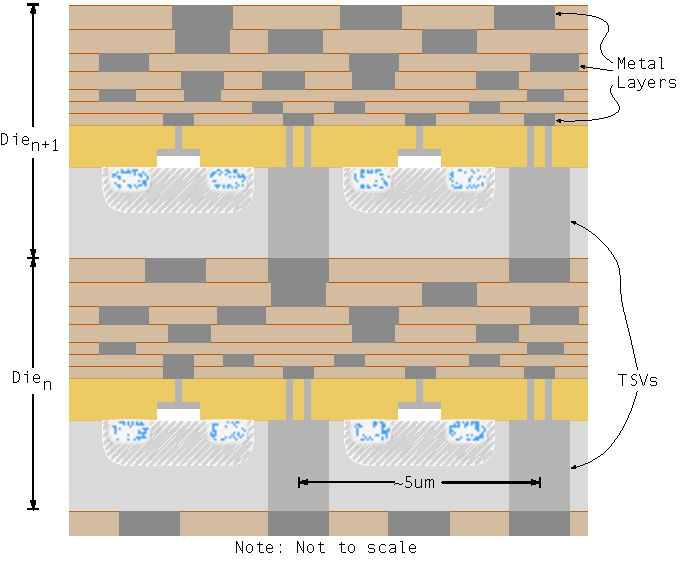
\includegraphics[width=4.5in]{TSVs.pdf}}
}
\caption{Die Stack profile \cite{itrs2015_interconn} with \acp{tsv}}
\label{fig:tsv}
\end{figure}

There are other definitions on how the dies are bonded together:
\begin{outline}
  \1 Wafer-to-Wafer
    \2 current \ac{esd} mitigation allows implementation of unbuffered IO
    \2 potential low yield because of lack of knowledge regarding \ac{kgd}
  \1 Die-to-Wafer
    \2 will need additional \ac{esd} mitigation support
    \2 higher yield because of knowledge of \ac{kgd}
  \1 Die-to-Die
    \2 will need additional \ac{esd} mitigation support
    \2 higher yield because of knowledge of \ac{kgd}
\end{outline}

This work is targeting \ac{3dic} technology that supports 3D-Stacked \ac{soc} or 3D-Stack \ac{ic} with high levels of interconnect.
To avoid using large IO buffers for the \ac{tsv} interconenct, this work assumes that the \ac{3dic} technology supports unbuffered interconnects. 
This would suggest wafer-to-wafer bonding because of the existing \ac{esd} mitigation during wafer handling although it is anticipated that improved \ac{esd} mitigation will be introduced in future manufacturing steps.

The technology roadmap in \cite{itrs2015_interconn} and the information in \cite{patti2014} suggests \SI{5}{\micro\meter} pitch \acp{tsv} is a reasonable design goal. This work assumes a one-to-one ration of signal \acp{tsv} to power/grod \ac{tsv} so when accounting for area associated with \acp{tsv}, the number of signal \acp{tsv} are doubled.

As a large amount of \acp{tsv} are employed, \ac{tsv} energy cannot be ignored.
Most of the energy dissipated in the \ac{tsv} is associated with the charging and discharging of the \acp{tsv} capacitance. For a \SI{5}{\micro\meter} pitch and \SI{2}{\micro\meter} radius \acp{tsv}, \cite{Bamberg2017} table I suggests an average capacitance of \SI{4.2}{\femto\farad} \footnote{\cite{tezzaron:preso} suggests a lower capacitance}.

Therefore, this work assumes \acp{tsv} with a \SI{5}{\micro\meter} pitch and a power dissipation of \SI[per-mode=symbol]{4.2}{\micro \watt \per \giga \bit\per\second \per \ac{tsv}}.







